% This is samplepaper.tex, a sample chapter demonstrating the
% LLNCS macro package for Springer Computer Science proceedings;
% Version 2.20 of 2017/10/04
%
\documentclass[runningheads]{llncs}

\usepackage{graphicx}
\usepackage{caption}
\usepackage{subfigure}
\usepackage[fleqn]{amsmath}
\usepackage[psamsfonts]{amssymb}
\usepackage{cite}
\begin{document}

\title{Optimizing the Computational Efficiency of 3D Segmentation Models for Connectomics}


\author{
Weihao Zhuang  %\inst{1} 
\and
Hascoet Tristan %\inst{1} 
\and
Ryoichi Takashima  %\inst{1}
\and
Tetsuya Takiguchi  %\inst{1}
\and
Yasuo Ariki %\inst{1}
}

\authorrunning{Weihao Zhuang et al.}

\institute{Graduate School of System Informatics, Kobe University, Japan}

\maketitle            

\begin{abstract}
The field of connectomics aims to map the interconnections between biological neurons within nervous systems at the scale of single synapses to gain insights into the structure and functional organization of biological neural networks. 
A critical task for the success of the connectomics enterprise is the segmentation of neurites from high precision electron microscopy (EM) images. 
This task requires models to be both accurate and computationally efficient in order to process large volumes of very high precision microscopy images. 
In recent years, deep learning based models have become very accurate at this task, at the cost of being very computationally intensive.
In this paper, we analyse the computational efficiency of one such successful model and identify several computational bottlenecks. 
We propose different optimizations to increase the computational efficiency of this model 
and achieve a 5 times speed up in computation time while slightly improving on the baseline model accuracy.

\keywords{Neurite segmentation  \and 3D CNN \and Computational efficiency}
\end{abstract}

\section{Introduction}
Precise reconstruction of neural connectivity is of great importance to understand the functional organization of biological nervous systems. 
3D electron microscopy (EM) can capture large volume of neuronal tissues within nano-scale precision, which allows for the identification of even the smallest neuronal objects like vesicles. 
With advances in imaging technologies, EM systems can now produce terabytes of images within hours. 
Manually annotating each of the neurons within such large EM volumes is simply impractical as it would require lifetimes of manual labeling from highly skilled experts to segment. 
Hence, high-precision segmentation models are needed to automate the reconstruction of neuronal circuits. 

\begin{figure}[h]
\centering
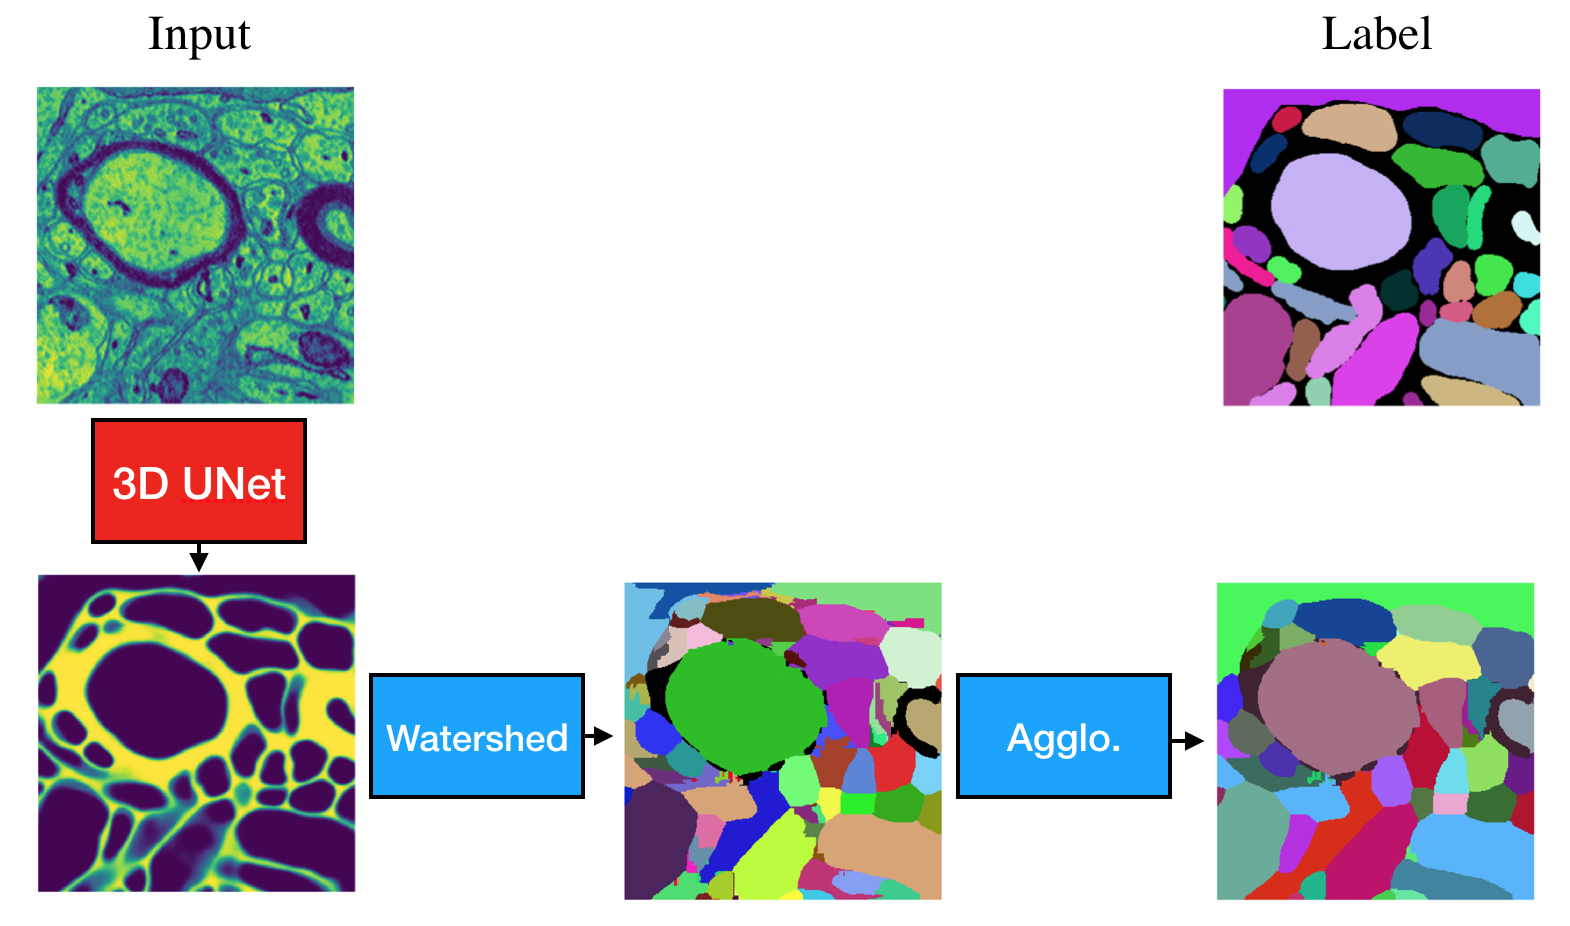
\includegraphics[width=2.8in]{Pipeline.png}
\caption{
Illustration of the 3-step segmentation pipeline. 
This paper focuses solely on increasing the computational efficiency of the first step.
}
\end{figure}

Current state-of-the art models for 3D neurite segmentation proceed in three steps, as illustrated in Figure 1. 
First, a CNN is trained to detect boundaries between neurons in the raw EM images. 
In a second step, over-segmentation maps are computed from the boundary map. 
This is typically done by non-parametric algorithms like Watershed. 
Finally, an agglomeration algorithm is used to process the over-segmented results typically produced by the Watershed algorithm. 

In this pipeline, the first step is computationally very expensive, 
both for the training step of the CNN and for the inference step.
The benefits of optimizing the computational efficiency of the 3D U-Net is two-folds: 

First, computationally efficient models would significantly ease the inference step: 
As the resolution needed to accurately detect synaptic connections is on the order of tens of nanometers,
only a cubic millimeter of brain tissue at this resolution represents on the order of PetaBytes. 
Processing such a large volume is a considerable computational challenge. 
Hence optimized computations will be needed in order to enable the processing of large brain volumes.

However, the most impactful benefit concerns the training step: 
As training an unoptimized model to convergence takes up to days on a single GPU machine, 
the iterative process needed to fine-tune our models 
and experiment with different architectures and loss functions is very slow. 
Hence, optimizing the computational efficiency of our model would enable us to more efficiently explore the space of possible solution, 
thanks to faster iteration cycles. 

In this paper, we thus analyse the computational efficiency of a successful 3D U-Net segmentation model
and identify different factors responsible for slowing down the computations. 
We propose several improvements to speed up the baseline computations and achieve a relative speed of up to 500\% 
without sacrifying the model accuracy.
In fact, through a better parameterization of the baseline model, 
we are able to achieve an improvement of 0.5\% in accuracy while speeding up the computations.  

In the next section, we start by analysing the baseline model. 
We present our proposed optimization in Section 3. 
Section 4 discusses the results of our experiments and Section 5 concludes this paper.

\section{Baseline model Analysis}

\subsection{Baseline model}

We chose the 3D U-Net proposed by Lee \textit{et al.} \cite{lee2017superhuman} as our baseline model to optimize.
This model, illustrated in Figure 2, was the first model to surpass human accuracy on the SNEMI3D challenge.
This model builds on the original U-Net architecture \cite{ronneberger2015u} and proposes several improvement:

\begin{figure}[h]
\centering
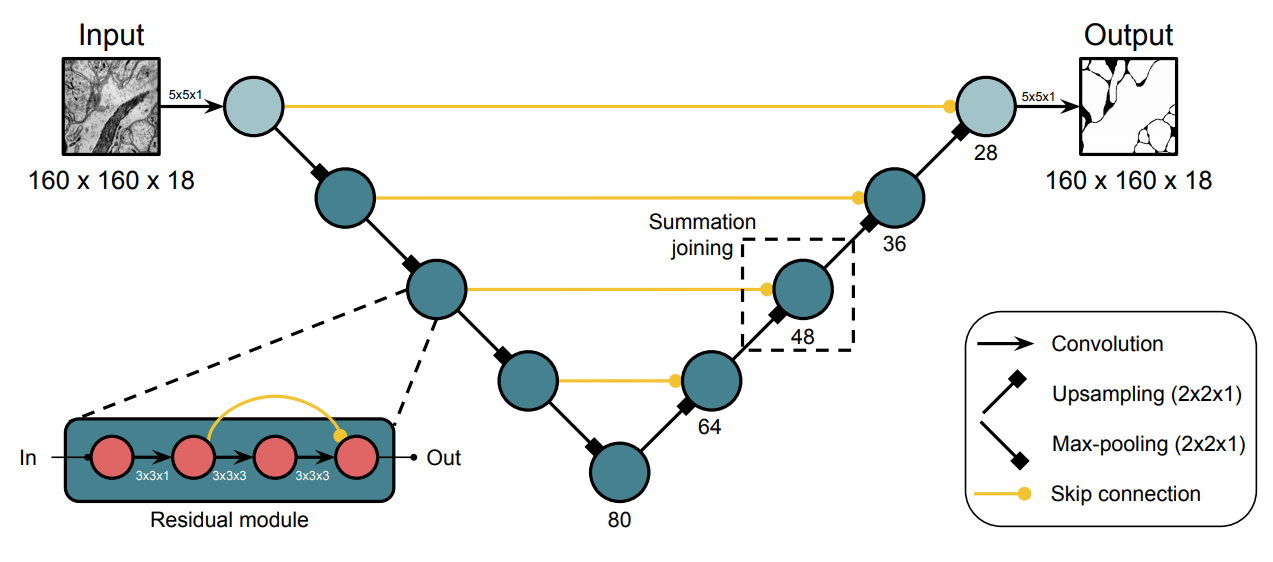
\includegraphics[width=2.8in]{Architecture.png}
\caption{
Illustration of the baseline model architecture (drawn from \cite{lee2017superhuman}). 
We adapt this architecture to the specific anisometry of our dataset 
by replacing the 2D sampling of lower layers by 3D sampling operations ($2 \times 2 \times 2$).
}
\end{figure}

First, skip connections are made by summation instead of concatenation,
so that the down-sampling and up-sampling pathes have the same number of channels.
Second, operations at each pooling level are standardized as a similar convolution block made of 
convolution, activation and batch normalization layers with skip connections.

As we fine-tune low-level computation kernels for each layer in the network,
the symmetry of this architecture considerably facilitates our optimization task
as computations at each level are standardized.

Finally, pooling operations are adapted so as to match the isometry of the dataset.
We only adapt their architecture to fit the anisotropy of our own dataset by 
replacing the 2D pooling operations of the lower layers by 3D pooling operations.

\subsection{Model analysis}

We start by analyzing the computational efficiency of our baseline model.
Figure 3 shows the processing time spent in each layer of the network.
The time $t(l)$ (in seconds $s$) required by a given layer $l$ to process an input batch 
can be decomposed into the number of operations (FLOP) $O(l)$ divided by the computational efficiency (FLOP/s) $E(l)$ of the layer:

$$t(l) = \frac{0(l)}{E(l)} $$

The total processing time T required by the model $M$ to process an input batch 
is equal to the sum of the computation time spent in each layer:

$$T = \sum_{l \in M} t(l)$$

Figure 3 shows the number of operations, the efficiency, and the processing time spent in each convolution layer of the baseline model in the order of their processing: 
the left-most value of each plot represents the input layer, followed by the next lower layer, up until the output layer represented by the right-most value of the plot.
In reality, batch normalization, ReLU, pooling and skip connections should be represented on these plots between each convolution.
However, as the computations are dominated by convolution layers, we consider these layers negligible and only show the analysis of convolutions for readability. 

\begin{figure}[h]
\centering
\subfigure[FLOP]{
\begin{minipage}[t]{0.33\linewidth}
\centering
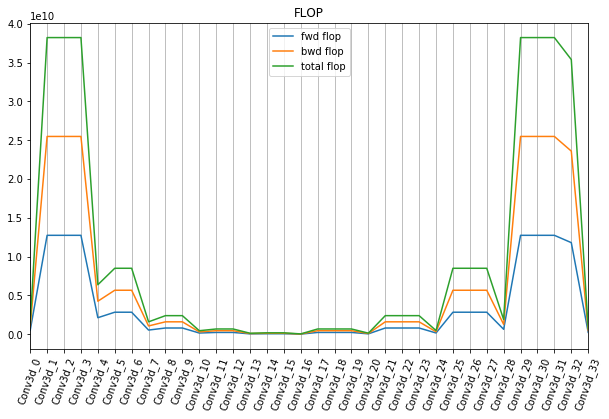
\includegraphics[width=1.6in]{FLOP.png}
%\caption{fig1}
\end{minipage}%
}%
\subfigure[FLOPs]{
\begin{minipage}[t]{0.33\linewidth}
\centering
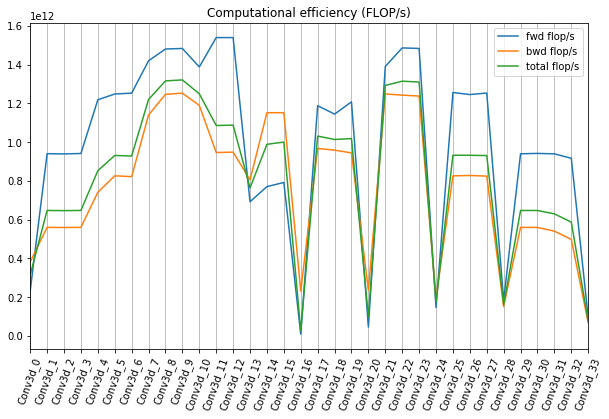
\includegraphics[width=1.6in]{FLOPs.png}
%\caption{fig2}
\end{minipage}%
}%
\subfigure[Time]{
\begin{minipage}[t]{0.33\linewidth}
\centering
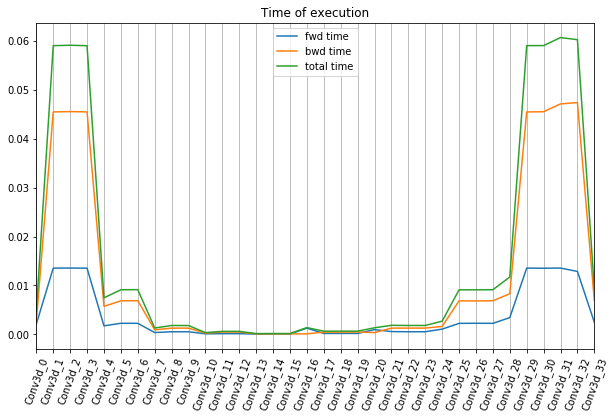
\includegraphics[width=1.6in]{Time.png}
%\caption{fig2}
\end{minipage}
}%
\centering
\caption{
Baseline model analysis. 
The $x$ axis, shared by all plots, represents the different convolution layers of the model in the order of their processing. 
(a) Number of operation $O(l)$ of each layer. 
(b) Computational efficiency $E(l)$ of each layer.
(c) Time $t(l)$ spent in the computation of each layer
For each layer, the computation of the forward pass is shown in blue, 
backward pass operations in yellow, 
while green measurments represent the full (forward + backward) operations
}
\end{figure}

\section{Baseline Model Optimization}

We minimize the total processing time $T$ by optimizing individual layers.
For a given layer $l$, minimizing the processing time $ t(l) $ can be achieved in two ways:
We can either reduce the number of operations $O(l)$ of a given layer $l$, or increase its efficiency $E(l)$.
Reducing the number of operations $O(l)$ is done by modifying the architecture parameters, which we explain in the following section.
Increasing the computational efficiency is done by optimizing the low-level implementation of the convolutions, which we explain in Section 3.2.

\subsection{Architectural optimization}

\begin{figure}[h]
\centering
\subfigure[ResNet]{
\begin{minipage}[t]{0.5\linewidth}
\centering
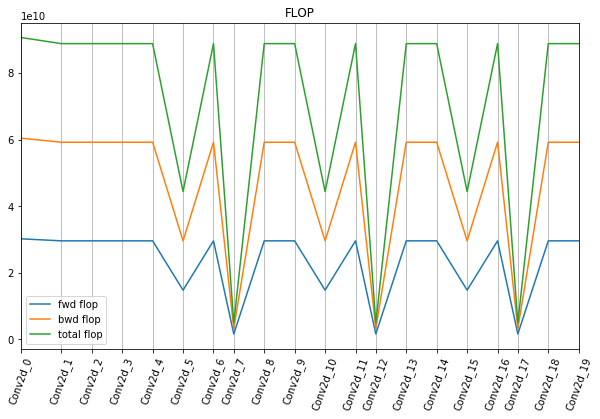
\includegraphics[width=2.3in]{2D_Resnet_FLOP.png}
%\caption{fig1}
\end{minipage}%
}%
\subfigure[3D UNet]{
\begin{minipage}[t]{0.5\linewidth}
\centering
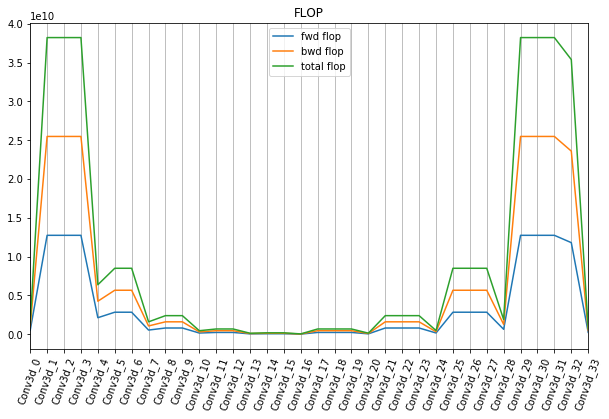
\includegraphics[width=2.3in]{FLOP.png}
%\caption{fig2}
\end{minipage}%
}%

\centering
\caption{FLOP distribution among the layers of two different models: (a) a 2D ResNet, and (b) the baseline 3D U-Net}
\end{figure}

Figure 4 compares the distribution of FLOP among each layers of a 2D ResNet \cite{he2016deep} and our baseline 3D UNet.

The 2D-ResNet computations are evenly distributed among its layers, while the 3D UNet computations concentrate on the 
first and last three layers of the network, which consume over 85\% of the total computational cost.
Intuitively, this seems misguided as there is no rational for the low level feature processing to be that much more computationally 
expensive than the higher level feature processing.
The 2D ResNet has been carefully parameterized so as to maintain a constant computational 
for convolutional layers across the full model:
In ResNets, the number of channels is doubled after each pooling layers, 
while pooling reduce each spatial dimension by a factor of 2.
The computational complexity (FLOP) of a convolution operation with stride 1 at layer $l$ is given by:

$$ O(l) = h \times w \times c^2 \times bs  \times kh  \times kw $$

Where $h,w$ represents the input image dimensions, 
the input and output channels $c$ are considered equal, 
and $kh,kw$ represent the spatial dimensions of the kernel.

Hence, the computational complexity is quadratic in both the input spatial dimension ($h \times w$),
and the channel dimension ($c^2$).
Denoting by $l'$ an upstream layer of $l$ after pooling, the computational complexity in ResNet parameterization is given by:


\begin{subequations} 
\begin{align}
O(l') &= h' \times w' \times c'^2 \times bs'  \times kh'  \times kw'  \\
O(l') &= (h/2) \times (w/2) \times (c \times 2)^2 \times bs  \times kh  \times kw   \\
O(l') &= h \times w \times c^2 \times bs  \times kh  \times kw   \\
O(l') &= O(l) 
\end{align}
\end{subequations}


Hence, by doubling the number of channels after each pooling operations, ResNet maintains a computational cost constant with depth.
To maintain a constant computational cost with depth, 3D CNNs should thus scale the channel dimension
by a factor of $\sqrt{2^3}=\sqrt{8}$ after each pooling operation, 
which is far more than the scaling factor used by the original baseline model.
This explains why the computational cost is concentrated in the first layers as 
it is exponentially decreased with depth.
We thus increase the channel scaling factor so as to maintain a constant computational cost in the first three pooling levels.

To further reduce the computational cost of the first and last layer, 
we draw inspiration from efficient ResNet implementations and replace the first and
last layer of our model by strided and fractionally strided convolutions respectively.
This allows us to minimize the amount of computation performed at full resolution.

\begin{figure}[h]
\centering
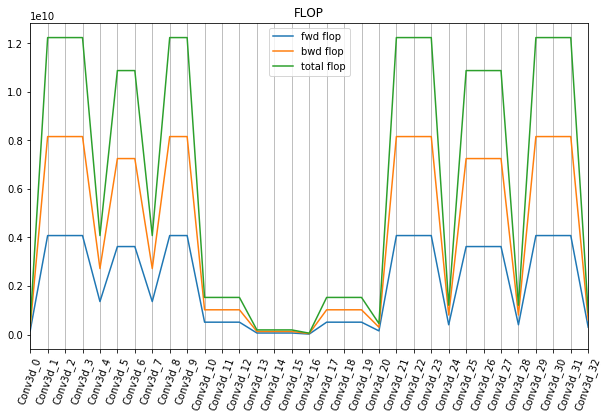
\includegraphics[width=2.8in]{optimize_model_FLOP.png}
\caption{FLOP optimization}
\end{figure}%

\subsection{Implementation optimization}

In this section, we describe the optimization of the computational efficiency $E(l)$ of the convolution layers of our network.
We do this by fine-tuning low-level GPU kernels tailored to our computational workload using AutoTVM \cite{chen2018tvm}.
The result of our optimization is shown in Figure 6.

%Cannot reach the maximum theoretical computational efficiency
We run our model on a Nvidia TITAN X, whose peak computation efficiency is 10 TFLOPs (illustrated in red in Figure 6) according to the official specification.
Compared to its theoretical performance, our baseline model implemented in PyTorch reached a peak performance below 4 TFLOPs,
which suggests plenty of room for optimization.

%use tvm to optimize computation, distange of cudnn, what is tvm, halide, autotvm 
Pytorch uses cuDNN as a backend for high efficiency GPU implementation of its operations.
cuDNN \cite{chetlur2014cudnn} is a handwritten low-level deep learning implement acceleration library, provided by NVIDIA for its GPUs. 
cuDNN kernels are hand-optimized kernels targetting specialized hardware and computational workloads. 
In contrast, AutoTVM \cite{chen2018tvm} recently proposed a machine learning-based optimization of low-level implementations 
allowing to fine-tune specific kernels to specific hardware and workloads.
We used AutoTVM to fine-tune low-level kernels for our model.
The per-layer efficiency achieved by AutoTVM is shown in Figure 6, and Table 1 summarizes the total increase in performance achieved by the full model.

\begin{figure}[h]
\centering
\subfigure[Pytorch (cuDNN kernel function)]{
\begin{minipage}[t]{0.5\linewidth}
\centering
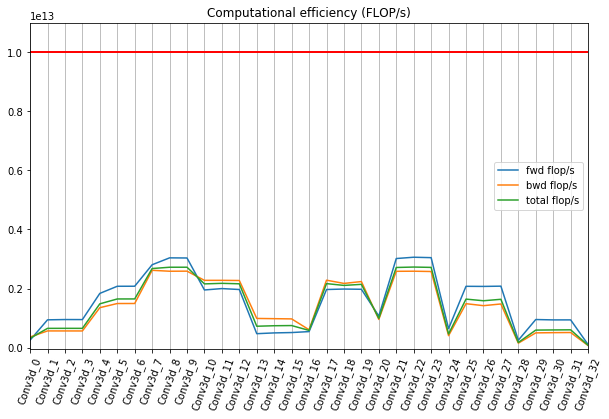
\includegraphics[width=2.3in]{optimize_model_FLOPs_peak_pytorch.png}
\end{minipage}
}
\subfigure[TVM (autotuing kernel function)]{
\begin{minipage}[t]{0.5\linewidth}
\centering
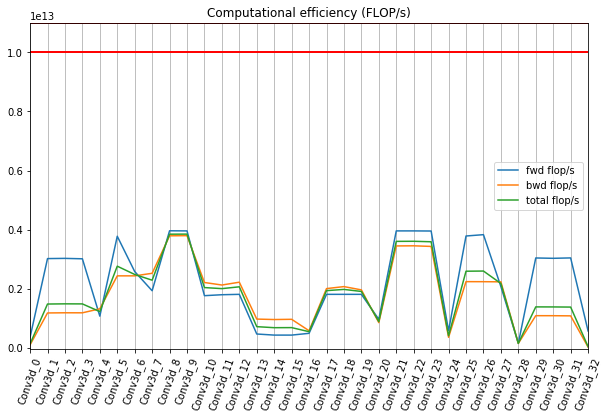
\includegraphics[width=2.3in]{optimize_model_FLOPs_peak_tvm.png}
\end{minipage}
}
\centering
\caption{Computational efficiency achieved by our model using (a) cudnn kernels and (b) custom AutoTVM kernels}
\end{figure}


\section{Experiment}



In this section, we evaluate the speed and accuracy of the baseline model after each modification proposed in the previous section.
Optimizing for computational speed involves a trade-off between speed and accuracy.
We expect architectural changes aiming to reduce the number of operations to increase speed at the expense of accuracy,
while implementation optimization should not impact the accuracy.
We start by describing the dataset used in these experiments, and present the results further below.

\subsection{Dataset}

We used the SNEMI3D dataset and rescaled it to an anisotropy factor of 2 in order 
to match the taget anisotropy allowed by our own imaging equipment.
We split the dataset along its $x$ axis, and use 80\% percent of the annotated volume as training data
with the remaining 20\% serving as validation set.

\subsection{Results}

In this section, we report the changes in accuracy and computational efficiency
brought by each of our proposed optimization. 
These results are presented in Table 1.

\begin{table}
% table caption is above the table
\centering
\caption{Experiment Results}
\label{tab:1}
\begin{tabular}{ccccccc}
\hline\noalign{\smallskip}
Stride & Channel & Implement & Accuracy & GFLOP & GFLOPs & Time(one iteration)  \\
\noalign{\smallskip}\hline\noalign{\smallskip}
No & 24, 32, 48, 72, 104 & Pytorch & 92.63\% &  430.66 & 607.25 & 0.71s\\
Yes & 24, 32, 48, 72, 104 & Pytorch & 92.57\% &  97.02 & 599.92 & 0.16s\\
Yes & 24, 64, 192, 192, 192 & Pytorch & 93.08\% &  211.24 & 983.35 & 0.21s\\
Yes & 24, 64, 192, 192, 192 & TVM & 93.08\% & 211.24 & \textbf{1627.13} &  \textbf{0.13s}\\
\noalign{\smallskip}\hline
\end{tabular}
\end{table}

First, replacing the first convolution layer with a strided convolution significantly decreases the computation time
as most of the computational cost of the original baseline was concentrated in the upper layers due to their high spatial resolution.
Surprisingly, this modification barely impacted the accuracy.
Second, we increase the channel dimension after each pooling layer to maintain a constant computational cost with depth.
This proved to increase the accuracy by $0.5$\%, while incurring a small computation overhead of $50$ ms per iteration.  
Finally, replacing the cuDNN kernel with customely fine-tuned kernels further reduced the computation time from 0.21s per iteration to 0.13s.

Taken together, our optimizations allowed to reduce the computation time from $0.71$s per iteration to $0.13$s, 
while increasing the model accuracy from $92.63$\% to $93.08$\%.

\subsection{Future Work}

We are still far from the optimal computational efficiency, 
since our experiment device can reach to 10 TFLOPs instead of 4 TFLOPs which is the peak computational efficiency achieved by our model.
In particular, the weight gradient computations of convolution layers remain too slow in our implementation.
We will continue to tune our scheduling implementations in order to further accelerate our model computations.
Furthermore, a number of recent advances in numerics and hardware have pushed the computation 
power of GPUs beyond tens of Teraflops.
These include mixed precision training and tensorized operations as allowed by the Tensor Core technology.
We plan to integrate these advancements to further boost the efficiency of our model in future research.

\section{Conclusion}

Neuroscience, and the connectomics endeavor in particular, can greatly benefit from automated neurite segmentation systems.
As the imaging resoltion required to properly analyze brain tissues is very high, analyzing large volume of brain tissues is computationally intensive task.
In this paper, we analyzed the computational efficiency of a baseline neurone segmentation model and proposed several improvements to accelerate its computations.
We manage to achieve a 5 times speed up while simultaneously improving on the baseline model accuracy.
Our analysis suggests that further gains are possible, which we will continue to investigate in future work.
%

% ---- Bibliography ----

%

% BibTeX users should specify bibliography style 'splncs04'.

% References will then be sorted and formatted in the correct style.

%
\bibliographystyle{splncs04}

\bibliography{samplepaper}


%

%\begin{thebibliography}{8}
%
%\bibitem{3D UNet}
%Lee, K., Zung, J., Li, P., Jain, V., & Seung, H. S. (2017). Superhuman accuracy on the SNEMI3D connectomics challenge. arXiv preprint arXiv:1706.00120.
%
%
%\bibitem{ref_lncs1}
%
%Author, F., Author, S.: Title of a proceedings paper. In: Editor,
%
%F., Editor, S. (eds.) CONFERENCE 2016, LNCS, vol. 9999, pp. 1--13.
%
%Springer, Heidelberg (2016). \doi{10.10007/1234567890}

%
%\end{thebibliography}


\end{document}
